\documentclass{standalone}
%\usepackage[margin=0.5in]{geometry}
\usepackage{tikz}
\usetikzlibrary{calc}

\begin{document}

% ---------- knobs ----------
\def\N{16}        % grid subdivisions per side
\def\Scale{4}    % overall size on the page (try 9.5–11)
% ---------------------------

\begin{tikzpicture}[scale=\Scale, line cap=round, line join=round]
  % precompute loop upper bound safely  
  \pgfmathtruncatemacro{\Nm}{\N-1}

  % unit equilateral triangle with decimal height (sqrt(3)/2 ≈ 0.8660254038)
  \coordinate (A) at (0,0);
  \coordinate (B) at (1,0);
  \coordinate (C) at (0.5,0.8660254038);

  % grid lines: three families
  \foreach \k in {1,...,\Nm} {
    \pgfmathsetmacro{\t}{\k/\N}

    % parallel to BC
    \draw[very thin, gray!55] ($(A)!\t!(B)$) -- ($(A)!\t!(C)$);

    % parallel to AC
    \draw[very thin, gray!55] ($(B)!\t!(A)$) -- ($(B)!\t!(C)$);

    % parallel to AB
    \draw[very thin, gray!55] ($(C)!\t!(A)$) -- ($(C)!\t!(B)$);
  }

  % border
  \draw[thick] (A)--(B)--(C)--cycle;

  % ticks (optional; comment out for blank paper)
  \foreach \k in {0,...,\N} {
    \pgfmathsetmacro{\t}{\k/\N}
    \draw[thin] ($(A)!\t!(B)$) -- ++(0,-0.015);
    \draw[thin] ($(A)!\t!(C)$) -- ++(-0.013,0.007);
    \draw[thin] ($(B)!\t!(C)$) -- ++(0.013,0.007);
  }

  % corner labels (optional)
  \node[below left]  at (A) {$(8,0,0)$};
  \node[below right] at (B) {$(0,8,0)$};
  \node[above]       at (C) {$(0,0,8)$};

  \coordinate (L) at ($ (A)!0.5!(B) $);
  \coordinate (M) at ($ (B)!0.5!(C) $);
  \coordinate (N) at ($ (C)!0.5!(A) $);

  \draw[fill=gray!20] (L)--(A)--(N)--cycle;
  \draw[fill=gray!20] (L)--(B)--(M)--cycle;
  \draw[fill=gray!20] (M)--(C)--(N)--cycle;


\end{tikzpicture}
\end{document}
%
\hfill
%
\begin{tikzpicture}[scale=\Scale, line cap=round, line join=round]
  % precompute loop upper bound safely
  \pgfmathtruncatemacro{\Nm}{\N-1}

  % unit equilateral triangle with decimal height (sqrt(3)/2 ≈ 0.8660254038)
  \coordinate (A) at (0,0);
  \coordinate (B) at (1,0);
  \coordinate (C) at (0.5,0.8660254038);

  % grid lines: three families
  \foreach \k in {1,...,\Nm} {
    \pgfmathsetmacro{\t}{\k/\N}

    % parallel to BC
    \draw[very thin, gray!55] ($(A)!\t!(B)$) -- ($(A)!\t!(C)$);

    % parallel to AC
    \draw[very thin, gray!55] ($(B)!\t!(A)$) -- ($(B)!\t!(C)$);

    % parallel to AB
    \draw[very thin, gray!55] ($(C)!\t!(A)$) -- ($(C)!\t!(B)$);
  }

  % border
  \draw[thick] (A)--(B)--(C)--cycle;

  % ticks (optional; comment out for blank paper)
  \foreach \k in {0,...,\N} {
    \pgfmathsetmacro{\t}{\k/\N}
    \draw[thin] ($(A)!\t!(B)$) -- ++(0,-0.015);
    \draw[thin] ($(A)!\t!(C)$) -- ++(-0.013,0.007);
    \draw[thin] ($(B)!\t!(C)$) -- ++(0.013,0.007);
  }

  % corner labels (optional)
  \node[below left]  at (A) {$(8,0,0)$};
  \node[below right] at (B) {$(0,8,0)$};
  \node[above]       at (C) {$(0,0,8)$};

  \coordinate (L) at ($ (A)!0.25!(B) $);
  \coordinate (X) at ($ (A)!0.75!(B) $);
  \coordinate (M) at ($ (B)!0.75!(C) $);
  \coordinate (Y) at ($ (B)!0.25!(C) $);
  \coordinate (N) at ($ (C)!0.75!(A) $);
  \coordinate (Z) at ($ (C)!0.25!(A) $);

  \draw[fill=gray!20] (L)--(A)--(N)--cycle;
  \draw[fill=gray!20] (X)--(B)--(Y)--cycle;
  \draw[fill=gray!20] (M)--(C)--(Z)--cycle;


\end{tikzpicture}
%
\hfill
%
\begin{tikzpicture}[scale=\Scale, line cap=round, line join=round]
  % precompute loop upper bound safely
  \pgfmathtruncatemacro{\Nm}{\N-1}

  % unit equilateral triangle with decimal height (sqrt(3)/2 ≈ 0.8660254038)
  \coordinate (A) at (0,0);
  \coordinate (B) at (1,0);
  \coordinate (C) at (0.5,0.8660254038);

  % grid lines: three families
  \foreach \k in {1,...,\Nm} {
    \pgfmathsetmacro{\t}{\k/\N}

    % parallel to BC
    \draw[very thin, gray!55] ($(A)!\t!(B)$) -- ($(A)!\t!(C)$);

    % parallel to AC
    \draw[very thin, gray!55] ($(B)!\t!(A)$) -- ($(B)!\t!(C)$);

    % parallel to AB
    \draw[very thin, gray!55] ($(C)!\t!(A)$) -- ($(C)!\t!(B)$);
  }

  % border
  \draw[thick] (A)--(B)--(C)--cycle;

  % ticks (optional; comment out for blank paper)
  \foreach \k in {0,...,\N} {
    \pgfmathsetmacro{\t}{\k/\N}
    \draw[thin] ($(A)!\t!(B)$) -- ++(0,-0.015);
    \draw[thin] ($(A)!\t!(C)$) -- ++(-0.013,0.007);
    \draw[thin] ($(B)!\t!(C)$) -- ++(0.013,0.007);
  }

  % corner labels (optional)
  \node[below left]  at (A) {$x$};
  \node[below right] at (B) {$y$};
  \node[above]       at (C) {$z$};

\end{tikzpicture}

\end{document}

\vfill

\clearpage

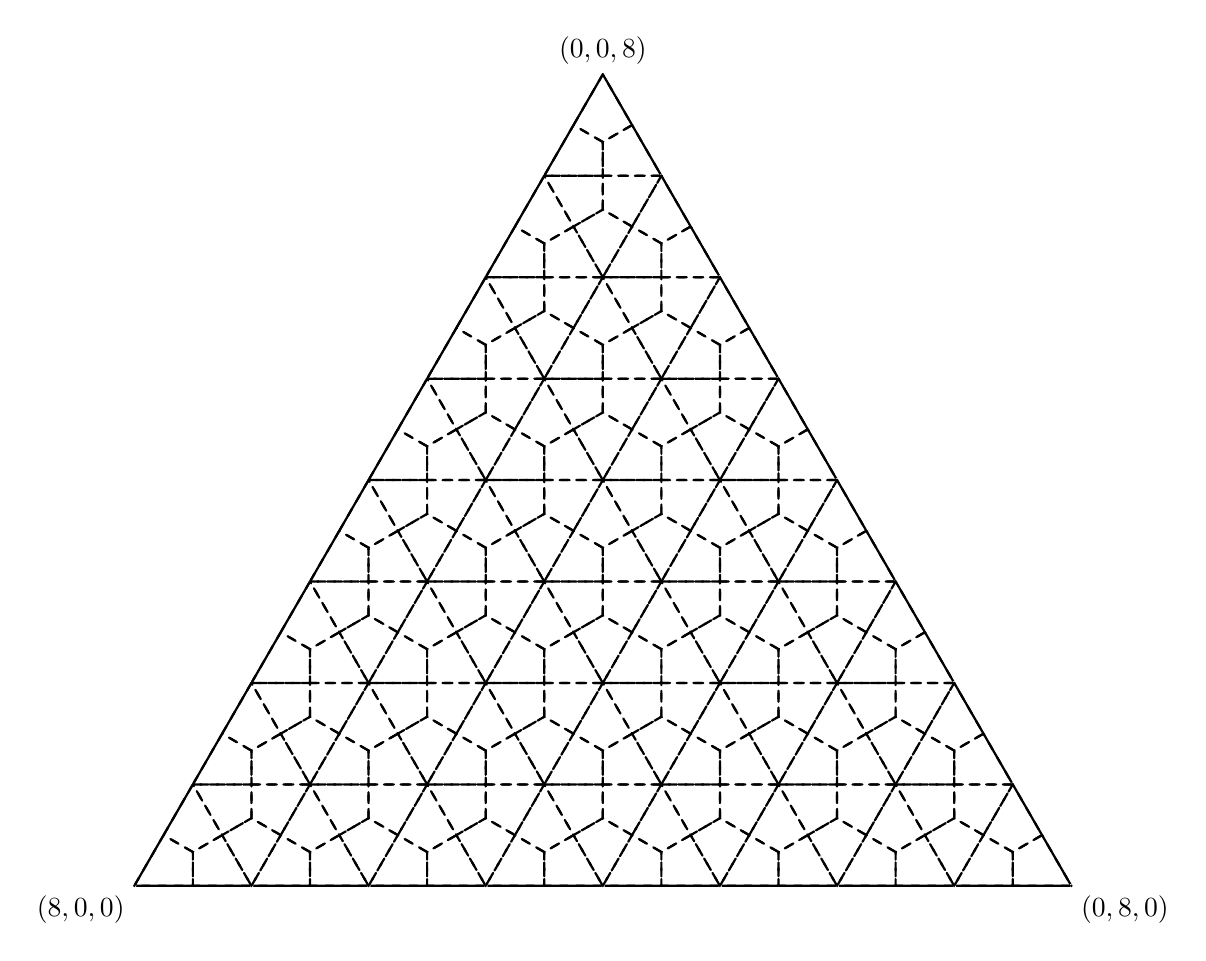
\begin{tikzpicture}[scale=0.7, line cap=round, line join=round]
  \def\N{8}
  \def\S{17.0}
  \coordinate (A) at (0,0);
  \coordinate (B) at (\S,0);
  \coordinate (C) at ({\S/2},{\S*sqrt(3)/2});
  \draw[thick] (A)--(B)--(C)--cycle;
  \node[below left] at (A) {$(\N,0,0)$};
  \node[below right] at (B) {$(0,\N,0)$};
  \node[above] at (C) {$(0,0,\N)$};
  % lattice points
  \fill[white] (8.500000,14.722432) circle (1.05pt);
  \fill[black] (8.500000,14.722432) circle (0.75pt);
  \fill[white] (9.562500,12.882128) circle (1.05pt);
  \fill[black] (9.562500,12.882128) circle (0.75pt);
  \fill[white] (10.625000,11.041824) circle (1.05pt);
  \fill[black] (10.625000,11.041824) circle (0.75pt);
  \fill[white] (11.687500,9.201520) circle (1.05pt);
  \fill[black] (11.687500,9.201520) circle (0.75pt);
  \fill[white] (12.750000,7.361216) circle (1.05pt);
  \fill[black] (12.750000,7.361216) circle (0.75pt);
  \fill[white] (13.812500,5.520912) circle (1.05pt);
  \fill[black] (13.812500,5.520912) circle (0.75pt);
  \fill[white] (14.875000,3.680608) circle (1.05pt);
  \fill[black] (14.875000,3.680608) circle (0.75pt);
  \fill[white] (15.937500,1.840304) circle (1.05pt);
  \fill[black] (15.937500,1.840304) circle (0.75pt);
  \fill[white] (17.000000,0.000000) circle (1.05pt);
  \fill[black] (17.000000,0.000000) circle (0.75pt);
  \fill[white] (7.437500,12.882128) circle (1.05pt);
  \fill[black] (7.437500,12.882128) circle (0.75pt);
  \fill[white] (8.500000,11.041824) circle (1.05pt);
  \fill[black] (8.500000,11.041824) circle (0.75pt);
  \fill[white] (9.562500,9.201520) circle (1.05pt);
  \fill[black] (9.562500,9.201520) circle (0.75pt);
  \fill[white] (10.625000,7.361216) circle (1.05pt);
  \fill[black] (10.625000,7.361216) circle (0.75pt);
  \fill[white] (11.687500,5.520912) circle (1.05pt);
  \fill[black] (11.687500,5.520912) circle (0.75pt);
  \fill[white] (12.750000,3.680608) circle (1.05pt);
  \fill[black] (12.750000,3.680608) circle (0.75pt);
  \fill[white] (13.812500,1.840304) circle (1.05pt);
  \fill[black] (13.812500,1.840304) circle (0.75pt);
  \fill[white] (14.875000,0.000000) circle (1.05pt);
  \fill[black] (14.875000,0.000000) circle (0.75pt);
  \fill[white] (6.375000,11.041824) circle (1.05pt);
  \fill[black] (6.375000,11.041824) circle (0.75pt);
  \fill[white] (7.437500,9.201520) circle (1.05pt);
  \fill[black] (7.437500,9.201520) circle (0.75pt);
  \fill[white] (8.500000,7.361216) circle (1.05pt);
  \fill[black] (8.500000,7.361216) circle (0.75pt);
  \fill[white] (9.562500,5.520912) circle (1.05pt);
  \fill[black] (9.562500,5.520912) circle (0.75pt);
  \fill[white] (10.625000,3.680608) circle (1.05pt);
  \fill[black] (10.625000,3.680608) circle (0.75pt);
  \fill[white] (11.687500,1.840304) circle (1.05pt);
  \fill[black] (11.687500,1.840304) circle (0.75pt);
  \fill[white] (12.750000,0.000000) circle (1.05pt);
  \fill[black] (12.750000,0.000000) circle (0.75pt);
  \fill[white] (5.312500,9.201520) circle (1.05pt);
  \fill[black] (5.312500,9.201520) circle (0.75pt);
  \fill[white] (6.375000,7.361216) circle (1.05pt);
  \fill[black] (6.375000,7.361216) circle (0.75pt);
  \fill[white] (7.437500,5.520912) circle (1.05pt);
  \fill[black] (7.437500,5.520912) circle (0.75pt);
  \fill[white] (8.500000,3.680608) circle (1.05pt);
  \fill[black] (8.500000,3.680608) circle (0.75pt);
  \fill[white] (9.562500,1.840304) circle (1.05pt);
  \fill[black] (9.562500,1.840304) circle (0.75pt);
  \fill[white] (10.625000,0.000000) circle (1.05pt);
  \fill[black] (10.625000,0.000000) circle (0.75pt);
  \fill[white] (4.250000,7.361216) circle (1.05pt);
  \fill[black] (4.250000,7.361216) circle (0.75pt);
  \fill[white] (5.312500,5.520912) circle (1.05pt);
  \fill[black] (5.312500,5.520912) circle (0.75pt);
  \fill[white] (6.375000,3.680608) circle (1.05pt);
  \fill[black] (6.375000,3.680608) circle (0.75pt);
  \fill[white] (7.437500,1.840304) circle (1.05pt);
  \fill[black] (7.437500,1.840304) circle (0.75pt);
  \fill[white] (8.500000,0.000000) circle (1.05pt);
  \fill[black] (8.500000,0.000000) circle (0.75pt);
  \fill[white] (3.187500,5.520912) circle (1.05pt);
  \fill[black] (3.187500,5.520912) circle (0.75pt);
  \fill[white] (4.250000,3.680608) circle (1.05pt);
  \fill[black] (4.250000,3.680608) circle (0.75pt);
  \fill[white] (5.312500,1.840304) circle (1.05pt);
  \fill[black] (5.312500,1.840304) circle (0.75pt);
  \fill[white] (6.375000,0.000000) circle (1.05pt);
  \fill[black] (6.375000,0.000000) circle (0.75pt);
  \fill[white] (2.125000,3.680608) circle (1.05pt);
  \fill[black] (2.125000,3.680608) circle (0.75pt);
  \fill[white] (3.187500,1.840304) circle (1.05pt);
  \fill[black] (3.187500,1.840304) circle (0.75pt);
  \fill[white] (4.250000,0.000000) circle (1.05pt);
  \fill[black] (4.250000,0.000000) circle (0.75pt);
  \fill[white] (1.062500,1.840304) circle (1.05pt);
  \fill[black] (1.062500,1.840304) circle (0.75pt);
  \fill[white] (2.125000,0.000000) circle (1.05pt);
  \fill[black] (2.125000,0.000000) circle (0.75pt);
  \fill[white] (0.000000,0.000000) circle (1.05pt);
  \fill[black] (0.000000,0.000000) circle (0.75pt);
  % Hamilton S-pieces
  \tikzset{piece/.style={thick, dashed}}
  % m=(0, 0, 8), S=(2,), floors=(0, 0, 7)
  \draw[piece] (8.500000,14.722432) -- (7.968750,13.802280) -- (8.500000,13.495563) -- (9.031250,13.802280) -- cycle;
  % m=(0, 1, 7), S=(1,), floors=(0, 0, 7)
  \draw[piece] (9.031250,13.802280) -- (8.500000,13.495563) -- (8.500000,12.882128) -- (9.562500,12.882128) -- cycle;
  % m=(0, 1, 7), S=(2,), floors=(0, 1, 6)
  \draw[piece] (9.562500,12.882128) -- (9.031250,11.961976) -- (9.562500,11.655259) -- (10.093750,11.961976) -- cycle;
  % m=(0, 1, 7), S=(1, 2), floors=(0, 0, 6)
  \draw[piece] (9.562500,12.882128) -- (8.500000,12.882128) -- (8.500000,12.268693) -- (9.031250,11.961976) -- cycle;
  % m=(0, 2, 6), S=(1,), floors=(0, 1, 6)
  \draw[piece] (10.093750,11.961976) -- (9.562500,11.655259) -- (9.562500,11.041824) -- (10.625000,11.041824) -- cycle;
  % m=(0, 2, 6), S=(2,), floors=(0, 2, 5)
  \draw[piece] (10.625000,11.041824) -- (10.093750,10.121672) -- (10.625000,9.814955) -- (11.156250,10.121672) -- cycle;
  % m=(0, 2, 6), S=(1, 2), floors=(0, 1, 5)
  \draw[piece] (10.625000,11.041824) -- (9.562500,11.041824) -- (9.562500,10.428389) -- (10.093750,10.121672) -- cycle;
  % m=(0, 3, 5), S=(1,), floors=(0, 2, 5)
  \draw[piece] (11.156250,10.121672) -- (10.625000,9.814955) -- (10.625000,9.201520) -- (11.687500,9.201520) -- cycle;
  % m=(0, 3, 5), S=(2,), floors=(0, 3, 4)
  \draw[piece] (11.687500,9.201520) -- (11.156250,8.281368) -- (11.687500,7.974651) -- (12.218750,8.281368) -- cycle;
  % m=(0, 3, 5), S=(1, 2), floors=(0, 2, 4)
  \draw[piece] (11.687500,9.201520) -- (10.625000,9.201520) -- (10.625000,8.588085) -- (11.156250,8.281368) -- cycle;
  % m=(0, 4, 4), S=(1,), floors=(0, 3, 4)
  \draw[piece] (12.218750,8.281368) -- (11.687500,7.974651) -- (11.687500,7.361216) -- (12.750000,7.361216) -- cycle;
  % m=(0, 4, 4), S=(2,), floors=(0, 4, 3)
  \draw[piece] (12.750000,7.361216) -- (12.218750,6.441064) -- (12.750000,6.134347) -- (13.281250,6.441064) -- cycle;
  % m=(0, 4, 4), S=(1, 2), floors=(0, 3, 3)
  \draw[piece] (12.750000,7.361216) -- (11.687500,7.361216) -- (11.687500,6.747781) -- (12.218750,6.441064) -- cycle;
  % m=(0, 5, 3), S=(1,), floors=(0, 4, 3)
  \draw[piece] (13.281250,6.441064) -- (12.750000,6.134347) -- (12.750000,5.520912) -- (13.812500,5.520912) -- cycle;
  % m=(0, 5, 3), S=(2,), floors=(0, 5, 2)
  \draw[piece] (13.812500,5.520912) -- (13.281250,4.600760) -- (13.812500,4.294043) -- (14.343750,4.600760) -- cycle;
  % m=(0, 5, 3), S=(1, 2), floors=(0, 4, 2)
  \draw[piece] (13.812500,5.520912) -- (12.750000,5.520912) -- (12.750000,4.907477) -- (13.281250,4.600760) -- cycle;
  % m=(0, 6, 2), S=(1,), floors=(0, 5, 2)
  \draw[piece] (14.343750,4.600760) -- (13.812500,4.294043) -- (13.812500,3.680608) -- (14.875000,3.680608) -- cycle;
  % m=(0, 6, 2), S=(2,), floors=(0, 6, 1)
  \draw[piece] (14.875000,3.680608) -- (14.343750,2.760456) -- (14.875000,2.453739) -- (15.406250,2.760456) -- cycle;
  % m=(0, 6, 2), S=(1, 2), floors=(0, 5, 1)
  \draw[piece] (14.875000,3.680608) -- (13.812500,3.680608) -- (13.812500,3.067173) -- (14.343750,2.760456) -- cycle;
  % m=(0, 7, 1), S=(1,), floors=(0, 6, 1)
  \draw[piece] (15.406250,2.760456) -- (14.875000,2.453739) -- (14.875000,1.840304) -- (15.937500,1.840304) -- cycle;
  % m=(0, 7, 1), S=(2,), floors=(0, 7, 0)
  \draw[piece] (15.937500,1.840304) -- (15.406250,0.920152) -- (15.937500,0.613435) -- (16.468750,0.920152) -- cycle;
  % m=(0, 7, 1), S=(1, 2), floors=(0, 6, 0)
  \draw[piece] (15.937500,1.840304) -- (14.875000,1.840304) -- (14.875000,1.226869) -- (15.406250,0.920152) -- cycle;
  % m=(0, 8, 0), S=(1,), floors=(0, 7, 0)
  \draw[piece] (16.468750,0.920152) -- (15.937500,0.613435) -- (15.937500,0.000000) -- (17.000000,0.000000) -- cycle;
  % m=(1, 0, 7), S=(0,), floors=(0, 0, 7)
  \draw[piece] (8.500000,13.495563) -- (7.968750,13.802280) -- (7.437500,12.882128) -- (8.500000,12.882128) -- cycle;
  % m=(1, 0, 7), S=(2,), floors=(1, 0, 6)
  \draw[piece] (7.437500,12.882128) -- (6.906250,11.961976) -- (7.437500,11.655259) -- (7.968750,11.961976) -- cycle;
  % m=(1, 0, 7), S=(0, 2), floors=(0, 0, 6)
  \draw[piece] (8.500000,12.882128) -- (7.437500,12.882128) -- (7.968750,11.961976) -- (8.500000,12.268693) -- cycle;
  % m=(1, 1, 6), S=(0,), floors=(0, 1, 6)
  \draw[piece] (9.562500,11.655259) -- (9.031250,11.961976) -- (8.500000,11.041824) -- (9.562500,11.041824) -- cycle;
  % m=(1, 1, 6), S=(1,), floors=(1, 0, 6)
  \draw[piece] (7.968750,11.961976) -- (7.437500,11.655259) -- (7.437500,11.041824) -- (8.500000,11.041824) -- cycle;
  % m=(1, 1, 6), S=(2,), floors=(1, 1, 5)
  \draw[piece] (8.500000,11.041824) -- (7.968750,10.121672) -- (8.500000,9.814955) -- (9.031250,10.121672) -- cycle;
  % m=(1, 1, 6), S=(0, 1), floors=(0, 0, 6)
  \draw[piece] (9.031250,11.961976) -- (8.500000,12.268693) -- (7.968750,11.961976) -- (8.500000,11.041824) -- cycle;
  % m=(1, 1, 6), S=(0, 2), floors=(0, 1, 5)
  \draw[piece] (9.562500,11.041824) -- (8.500000,11.041824) -- (9.031250,10.121672) -- (9.562500,10.428389) -- cycle;
  % m=(1, 1, 6), S=(1, 2), floors=(1, 0, 5)
  \draw[piece] (8.500000,11.041824) -- (7.437500,11.041824) -- (7.437500,10.428389) -- (7.968750,10.121672) -- cycle;
  % m=(1, 2, 5), S=(0,), floors=(0, 2, 5)
  \draw[piece] (10.625000,9.814955) -- (10.093750,10.121672) -- (9.562500,9.201520) -- (10.625000,9.201520) -- cycle;
  % m=(1, 2, 5), S=(1,), floors=(1, 1, 5)
  \draw[piece] (9.031250,10.121672) -- (8.500000,9.814955) -- (8.500000,9.201520) -- (9.562500,9.201520) -- cycle;
  % m=(1, 2, 5), S=(2,), floors=(1, 2, 4)
  \draw[piece] (9.562500,9.201520) -- (9.031250,8.281368) -- (9.562500,7.974651) -- (10.093750,8.281368) -- cycle;
  % m=(1, 2, 5), S=(0, 1), floors=(0, 1, 5)
  \draw[piece] (10.093750,10.121672) -- (9.562500,10.428389) -- (9.031250,10.121672) -- (9.562500,9.201520) -- cycle;
  % m=(1, 2, 5), S=(0, 2), floors=(0, 2, 4)
  \draw[piece] (10.625000,9.201520) -- (9.562500,9.201520) -- (10.093750,8.281368) -- (10.625000,8.588085) -- cycle;
  % m=(1, 2, 5), S=(1, 2), floors=(1, 1, 4)
  \draw[piece] (9.562500,9.201520) -- (8.500000,9.201520) -- (8.500000,8.588085) -- (9.031250,8.281368) -- cycle;
  % m=(1, 3, 4), S=(0,), floors=(0, 3, 4)
  \draw[piece] (11.687500,7.974651) -- (11.156250,8.281368) -- (10.625000,7.361216) -- (11.687500,7.361216) -- cycle;
  % m=(1, 3, 4), S=(1,), floors=(1, 2, 4)
  \draw[piece] (10.093750,8.281368) -- (9.562500,7.974651) -- (9.562500,7.361216) -- (10.625000,7.361216) -- cycle;
  % m=(1, 3, 4), S=(2,), floors=(1, 3, 3)
  \draw[piece] (10.625000,7.361216) -- (10.093750,6.441064) -- (10.625000,6.134347) -- (11.156250,6.441064) -- cycle;
  % m=(1, 3, 4), S=(0, 1), floors=(0, 2, 4)
  \draw[piece] (11.156250,8.281368) -- (10.625000,8.588085) -- (10.093750,8.281368) -- (10.625000,7.361216) -- cycle;
  % m=(1, 3, 4), S=(0, 2), floors=(0, 3, 3)
  \draw[piece] (11.687500,7.361216) -- (10.625000,7.361216) -- (11.156250,6.441064) -- (11.687500,6.747781) -- cycle;
  % m=(1, 3, 4), S=(1, 2), floors=(1, 2, 3)
  \draw[piece] (10.625000,7.361216) -- (9.562500,7.361216) -- (9.562500,6.747781) -- (10.093750,6.441064) -- cycle;
  % m=(1, 4, 3), S=(0,), floors=(0, 4, 3)
  \draw[piece] (12.750000,6.134347) -- (12.218750,6.441064) -- (11.687500,5.520912) -- (12.750000,5.520912) -- cycle;
  % m=(1, 4, 3), S=(1,), floors=(1, 3, 3)
  \draw[piece] (11.156250,6.441064) -- (10.625000,6.134347) -- (10.625000,5.520912) -- (11.687500,5.520912) -- cycle;
  % m=(1, 4, 3), S=(2,), floors=(1, 4, 2)
  \draw[piece] (11.687500,5.520912) -- (11.156250,4.600760) -- (11.687500,4.294043) -- (12.218750,4.600760) -- cycle;
  % m=(1, 4, 3), S=(0, 1), floors=(0, 3, 3)
  \draw[piece] (12.218750,6.441064) -- (11.687500,6.747781) -- (11.156250,6.441064) -- (11.687500,5.520912) -- cycle;
  % m=(1, 4, 3), S=(0, 2), floors=(0, 4, 2)
  \draw[piece] (12.750000,5.520912) -- (11.687500,5.520912) -- (12.218750,4.600760) -- (12.750000,4.907477) -- cycle;
  % m=(1, 4, 3), S=(1, 2), floors=(1, 3, 2)
  \draw[piece] (11.687500,5.520912) -- (10.625000,5.520912) -- (10.625000,4.907477) -- (11.156250,4.600760) -- cycle;
  % m=(1, 5, 2), S=(0,), floors=(0, 5, 2)
  \draw[piece] (13.812500,4.294043) -- (13.281250,4.600760) -- (12.750000,3.680608) -- (13.812500,3.680608) -- cycle;
  % m=(1, 5, 2), S=(1,), floors=(1, 4, 2)
  \draw[piece] (12.218750,4.600760) -- (11.687500,4.294043) -- (11.687500,3.680608) -- (12.750000,3.680608) -- cycle;
  % m=(1, 5, 2), S=(2,), floors=(1, 5, 1)
  \draw[piece] (12.750000,3.680608) -- (12.218750,2.760456) -- (12.750000,2.453739) -- (13.281250,2.760456) -- cycle;
  % m=(1, 5, 2), S=(0, 1), floors=(0, 4, 2)
  \draw[piece] (13.281250,4.600760) -- (12.750000,4.907477) -- (12.218750,4.600760) -- (12.750000,3.680608) -- cycle;
  % m=(1, 5, 2), S=(0, 2), floors=(0, 5, 1)
  \draw[piece] (13.812500,3.680608) -- (12.750000,3.680608) -- (13.281250,2.760456) -- (13.812500,3.067173) -- cycle;
  % m=(1, 5, 2), S=(1, 2), floors=(1, 4, 1)
  \draw[piece] (12.750000,3.680608) -- (11.687500,3.680608) -- (11.687500,3.067173) -- (12.218750,2.760456) -- cycle;
  % m=(1, 6, 1), S=(0,), floors=(0, 6, 1)
  \draw[piece] (14.875000,2.453739) -- (14.343750,2.760456) -- (13.812500,1.840304) -- (14.875000,1.840304) -- cycle;
  % m=(1, 6, 1), S=(1,), floors=(1, 5, 1)
  \draw[piece] (13.281250,2.760456) -- (12.750000,2.453739) -- (12.750000,1.840304) -- (13.812500,1.840304) -- cycle;
  % m=(1, 6, 1), S=(2,), floors=(1, 6, 0)
  \draw[piece] (13.812500,1.840304) -- (13.281250,0.920152) -- (13.812500,0.613435) -- (14.343750,0.920152) -- cycle;
  % m=(1, 6, 1), S=(0, 1), floors=(0, 5, 1)
  \draw[piece] (14.343750,2.760456) -- (13.812500,3.067173) -- (13.281250,2.760456) -- (13.812500,1.840304) -- cycle;
  % m=(1, 6, 1), S=(0, 2), floors=(0, 6, 0)
  \draw[piece] (14.875000,1.840304) -- (13.812500,1.840304) -- (14.343750,0.920152) -- (14.875000,1.226869) -- cycle;
  % m=(1, 6, 1), S=(1, 2), floors=(1, 5, 0)
  \draw[piece] (13.812500,1.840304) -- (12.750000,1.840304) -- (12.750000,1.226869) -- (13.281250,0.920152) -- cycle;
  % m=(1, 7, 0), S=(0,), floors=(0, 7, 0)
  \draw[piece] (15.937500,0.613435) -- (15.406250,0.920152) -- (14.875000,0.000000) -- (15.937500,0.000000) -- cycle;
  % m=(1, 7, 0), S=(1,), floors=(1, 6, 0)
  \draw[piece] (14.343750,0.920152) -- (13.812500,0.613435) -- (13.812500,0.000000) -- (14.875000,0.000000) -- cycle;
  % m=(1, 7, 0), S=(0, 1), floors=(0, 6, 0)
  \draw[piece] (15.406250,0.920152) -- (14.875000,1.226869) -- (14.343750,0.920152) -- (14.875000,0.000000) -- cycle;
  % m=(2, 0, 6), S=(0,), floors=(1, 0, 6)
  \draw[piece] (7.437500,11.655259) -- (6.906250,11.961976) -- (6.375000,11.041824) -- (7.437500,11.041824) -- cycle;
  % m=(2, 0, 6), S=(2,), floors=(2, 0, 5)
  \draw[piece] (6.375000,11.041824) -- (5.843750,10.121672) -- (6.375000,9.814955) -- (6.906250,10.121672) -- cycle;
  % m=(2, 0, 6), S=(0, 2), floors=(1, 0, 5)
  \draw[piece] (7.437500,11.041824) -- (6.375000,11.041824) -- (6.906250,10.121672) -- (7.437500,10.428389) -- cycle;
  % m=(2, 1, 5), S=(0,), floors=(1, 1, 5)
  \draw[piece] (8.500000,9.814955) -- (7.968750,10.121672) -- (7.437500,9.201520) -- (8.500000,9.201520) -- cycle;
  % m=(2, 1, 5), S=(1,), floors=(2, 0, 5)
  \draw[piece] (6.906250,10.121672) -- (6.375000,9.814955) -- (6.375000,9.201520) -- (7.437500,9.201520) -- cycle;
  % m=(2, 1, 5), S=(2,), floors=(2, 1, 4)
  \draw[piece] (7.437500,9.201520) -- (6.906250,8.281368) -- (7.437500,7.974651) -- (7.968750,8.281368) -- cycle;
  % m=(2, 1, 5), S=(0, 1), floors=(1, 0, 5)
  \draw[piece] (7.968750,10.121672) -- (7.437500,10.428389) -- (6.906250,10.121672) -- (7.437500,9.201520) -- cycle;
  % m=(2, 1, 5), S=(0, 2), floors=(1, 1, 4)
  \draw[piece] (8.500000,9.201520) -- (7.437500,9.201520) -- (7.968750,8.281368) -- (8.500000,8.588085) -- cycle;
  % m=(2, 1, 5), S=(1, 2), floors=(2, 0, 4)
  \draw[piece] (7.437500,9.201520) -- (6.375000,9.201520) -- (6.375000,8.588085) -- (6.906250,8.281368) -- cycle;
  % m=(2, 2, 4), S=(0,), floors=(1, 2, 4)
  \draw[piece] (9.562500,7.974651) -- (9.031250,8.281368) -- (8.500000,7.361216) -- (9.562500,7.361216) -- cycle;
  % m=(2, 2, 4), S=(1,), floors=(2, 1, 4)
  \draw[piece] (7.968750,8.281368) -- (7.437500,7.974651) -- (7.437500,7.361216) -- (8.500000,7.361216) -- cycle;
  % m=(2, 2, 4), S=(2,), floors=(2, 2, 3)
  \draw[piece] (8.500000,7.361216) -- (7.968750,6.441064) -- (8.500000,6.134347) -- (9.031250,6.441064) -- cycle;
  % m=(2, 2, 4), S=(0, 1), floors=(1, 1, 4)
  \draw[piece] (9.031250,8.281368) -- (8.500000,8.588085) -- (7.968750,8.281368) -- (8.500000,7.361216) -- cycle;
  % m=(2, 2, 4), S=(0, 2), floors=(1, 2, 3)
  \draw[piece] (9.562500,7.361216) -- (8.500000,7.361216) -- (9.031250,6.441064) -- (9.562500,6.747781) -- cycle;
  % m=(2, 2, 4), S=(1, 2), floors=(2, 1, 3)
  \draw[piece] (8.500000,7.361216) -- (7.437500,7.361216) -- (7.437500,6.747781) -- (7.968750,6.441064) -- cycle;
  % m=(2, 3, 3), S=(0,), floors=(1, 3, 3)
  \draw[piece] (10.625000,6.134347) -- (10.093750,6.441064) -- (9.562500,5.520912) -- (10.625000,5.520912) -- cycle;
  % m=(2, 3, 3), S=(1,), floors=(2, 2, 3)
  \draw[piece] (9.031250,6.441064) -- (8.500000,6.134347) -- (8.500000,5.520912) -- (9.562500,5.520912) -- cycle;
  % m=(2, 3, 3), S=(2,), floors=(2, 3, 2)
  \draw[piece] (9.562500,5.520912) -- (9.031250,4.600760) -- (9.562500,4.294043) -- (10.093750,4.600760) -- cycle;
  % m=(2, 3, 3), S=(0, 1), floors=(1, 2, 3)
  \draw[piece] (10.093750,6.441064) -- (9.562500,6.747781) -- (9.031250,6.441064) -- (9.562500,5.520912) -- cycle;
  % m=(2, 3, 3), S=(0, 2), floors=(1, 3, 2)
  \draw[piece] (10.625000,5.520912) -- (9.562500,5.520912) -- (10.093750,4.600760) -- (10.625000,4.907477) -- cycle;
  % m=(2, 3, 3), S=(1, 2), floors=(2, 2, 2)
  \draw[piece] (9.562500,5.520912) -- (8.500000,5.520912) -- (8.500000,4.907477) -- (9.031250,4.600760) -- cycle;
  % m=(2, 4, 2), S=(0,), floors=(1, 4, 2)
  \draw[piece] (11.687500,4.294043) -- (11.156250,4.600760) -- (10.625000,3.680608) -- (11.687500,3.680608) -- cycle;
  % m=(2, 4, 2), S=(1,), floors=(2, 3, 2)
  \draw[piece] (10.093750,4.600760) -- (9.562500,4.294043) -- (9.562500,3.680608) -- (10.625000,3.680608) -- cycle;
  % m=(2, 4, 2), S=(2,), floors=(2, 4, 1)
  \draw[piece] (10.625000,3.680608) -- (10.093750,2.760456) -- (10.625000,2.453739) -- (11.156250,2.760456) -- cycle;
  % m=(2, 4, 2), S=(0, 1), floors=(1, 3, 2)
  \draw[piece] (11.156250,4.600760) -- (10.625000,4.907477) -- (10.093750,4.600760) -- (10.625000,3.680608) -- cycle;
  % m=(2, 4, 2), S=(0, 2), floors=(1, 4, 1)
  \draw[piece] (11.687500,3.680608) -- (10.625000,3.680608) -- (11.156250,2.760456) -- (11.687500,3.067173) -- cycle;
  % m=(2, 4, 2), S=(1, 2), floors=(2, 3, 1)
  \draw[piece] (10.625000,3.680608) -- (9.562500,3.680608) -- (9.562500,3.067173) -- (10.093750,2.760456) -- cycle;
  % m=(2, 5, 1), S=(0,), floors=(1, 5, 1)
  \draw[piece] (12.750000,2.453739) -- (12.218750,2.760456) -- (11.687500,1.840304) -- (12.750000,1.840304) -- cycle;
  % m=(2, 5, 1), S=(1,), floors=(2, 4, 1)
  \draw[piece] (11.156250,2.760456) -- (10.625000,2.453739) -- (10.625000,1.840304) -- (11.687500,1.840304) -- cycle;
  % m=(2, 5, 1), S=(2,), floors=(2, 5, 0)
  \draw[piece] (11.687500,1.840304) -- (11.156250,0.920152) -- (11.687500,0.613435) -- (12.218750,0.920152) -- cycle;
  % m=(2, 5, 1), S=(0, 1), floors=(1, 4, 1)
  \draw[piece] (12.218750,2.760456) -- (11.687500,3.067173) -- (11.156250,2.760456) -- (11.687500,1.840304) -- cycle;
  % m=(2, 5, 1), S=(0, 2), floors=(1, 5, 0)
  \draw[piece] (12.750000,1.840304) -- (11.687500,1.840304) -- (12.218750,0.920152) -- (12.750000,1.226869) -- cycle;
  % m=(2, 5, 1), S=(1, 2), floors=(2, 4, 0)
  \draw[piece] (11.687500,1.840304) -- (10.625000,1.840304) -- (10.625000,1.226869) -- (11.156250,0.920152) -- cycle;
  % m=(2, 6, 0), S=(0,), floors=(1, 6, 0)
  \draw[piece] (13.812500,0.613435) -- (13.281250,0.920152) -- (12.750000,0.000000) -- (13.812500,0.000000) -- cycle;
  % m=(2, 6, 0), S=(1,), floors=(2, 5, 0)
  \draw[piece] (12.218750,0.920152) -- (11.687500,0.613435) -- (11.687500,0.000000) -- (12.750000,0.000000) -- cycle;
  % m=(2, 6, 0), S=(0, 1), floors=(1, 5, 0)
  \draw[piece] (13.281250,0.920152) -- (12.750000,1.226869) -- (12.218750,0.920152) -- (12.750000,0.000000) -- cycle;
  % m=(3, 0, 5), S=(0,), floors=(2, 0, 5)
  \draw[piece] (6.375000,9.814955) -- (5.843750,10.121672) -- (5.312500,9.201520) -- (6.375000,9.201520) -- cycle;
  % m=(3, 0, 5), S=(2,), floors=(3, 0, 4)
  \draw[piece] (5.312500,9.201520) -- (4.781250,8.281368) -- (5.312500,7.974651) -- (5.843750,8.281368) -- cycle;
  % m=(3, 0, 5), S=(0, 2), floors=(2, 0, 4)
  \draw[piece] (6.375000,9.201520) -- (5.312500,9.201520) -- (5.843750,8.281368) -- (6.375000,8.588085) -- cycle;
  % m=(3, 1, 4), S=(0,), floors=(2, 1, 4)
  \draw[piece] (7.437500,7.974651) -- (6.906250,8.281368) -- (6.375000,7.361216) -- (7.437500,7.361216) -- cycle;
  % m=(3, 1, 4), S=(1,), floors=(3, 0, 4)
  \draw[piece] (5.843750,8.281368) -- (5.312500,7.974651) -- (5.312500,7.361216) -- (6.375000,7.361216) -- cycle;
  % m=(3, 1, 4), S=(2,), floors=(3, 1, 3)
  \draw[piece] (6.375000,7.361216) -- (5.843750,6.441064) -- (6.375000,6.134347) -- (6.906250,6.441064) -- cycle;
  % m=(3, 1, 4), S=(0, 1), floors=(2, 0, 4)
  \draw[piece] (6.906250,8.281368) -- (6.375000,8.588085) -- (5.843750,8.281368) -- (6.375000,7.361216) -- cycle;
  % m=(3, 1, 4), S=(0, 2), floors=(2, 1, 3)
  \draw[piece] (7.437500,7.361216) -- (6.375000,7.361216) -- (6.906250,6.441064) -- (7.437500,6.747781) -- cycle;
  % m=(3, 1, 4), S=(1, 2), floors=(3, 0, 3)
  \draw[piece] (6.375000,7.361216) -- (5.312500,7.361216) -- (5.312500,6.747781) -- (5.843750,6.441064) -- cycle;
  % m=(3, 2, 3), S=(0,), floors=(2, 2, 3)
  \draw[piece] (8.500000,6.134347) -- (7.968750,6.441064) -- (7.437500,5.520912) -- (8.500000,5.520912) -- cycle;
  % m=(3, 2, 3), S=(1,), floors=(3, 1, 3)
  \draw[piece] (6.906250,6.441064) -- (6.375000,6.134347) -- (6.375000,5.520912) -- (7.437500,5.520912) -- cycle;
  % m=(3, 2, 3), S=(2,), floors=(3, 2, 2)
  \draw[piece] (7.437500,5.520912) -- (6.906250,4.600760) -- (7.437500,4.294043) -- (7.968750,4.600760) -- cycle;
  % m=(3, 2, 3), S=(0, 1), floors=(2, 1, 3)
  \draw[piece] (7.968750,6.441064) -- (7.437500,6.747781) -- (6.906250,6.441064) -- (7.437500,5.520912) -- cycle;
  % m=(3, 2, 3), S=(0, 2), floors=(2, 2, 2)
  \draw[piece] (8.500000,5.520912) -- (7.437500,5.520912) -- (7.968750,4.600760) -- (8.500000,4.907477) -- cycle;
  % m=(3, 2, 3), S=(1, 2), floors=(3, 1, 2)
  \draw[piece] (7.437500,5.520912) -- (6.375000,5.520912) -- (6.375000,4.907477) -- (6.906250,4.600760) -- cycle;
  % m=(3, 3, 2), S=(0,), floors=(2, 3, 2)
  \draw[piece] (9.562500,4.294043) -- (9.031250,4.600760) -- (8.500000,3.680608) -- (9.562500,3.680608) -- cycle;
  % m=(3, 3, 2), S=(1,), floors=(3, 2, 2)
  \draw[piece] (7.968750,4.600760) -- (7.437500,4.294043) -- (7.437500,3.680608) -- (8.500000,3.680608) -- cycle;
  % m=(3, 3, 2), S=(2,), floors=(3, 3, 1)
  \draw[piece] (8.500000,3.680608) -- (7.968750,2.760456) -- (8.500000,2.453739) -- (9.031250,2.760456) -- cycle;
  % m=(3, 3, 2), S=(0, 1), floors=(2, 2, 2)
  \draw[piece] (9.031250,4.600760) -- (8.500000,4.907477) -- (7.968750,4.600760) -- (8.500000,3.680608) -- cycle;
  % m=(3, 3, 2), S=(0, 2), floors=(2, 3, 1)
  \draw[piece] (9.562500,3.680608) -- (8.500000,3.680608) -- (9.031250,2.760456) -- (9.562500,3.067173) -- cycle;
  % m=(3, 3, 2), S=(1, 2), floors=(3, 2, 1)
  \draw[piece] (8.500000,3.680608) -- (7.437500,3.680608) -- (7.437500,3.067173) -- (7.968750,2.760456) -- cycle;
  % m=(3, 4, 1), S=(0,), floors=(2, 4, 1)
  \draw[piece] (10.625000,2.453739) -- (10.093750,2.760456) -- (9.562500,1.840304) -- (10.625000,1.840304) -- cycle;
  % m=(3, 4, 1), S=(1,), floors=(3, 3, 1)
  \draw[piece] (9.031250,2.760456) -- (8.500000,2.453739) -- (8.500000,1.840304) -- (9.562500,1.840304) -- cycle;
  % m=(3, 4, 1), S=(2,), floors=(3, 4, 0)
  \draw[piece] (9.562500,1.840304) -- (9.031250,0.920152) -- (9.562500,0.613435) -- (10.093750,0.920152) -- cycle;
  % m=(3, 4, 1), S=(0, 1), floors=(2, 3, 1)
  \draw[piece] (10.093750,2.760456) -- (9.562500,3.067173) -- (9.031250,2.760456) -- (9.562500,1.840304) -- cycle;
  % m=(3, 4, 1), S=(0, 2), floors=(2, 4, 0)
  \draw[piece] (10.625000,1.840304) -- (9.562500,1.840304) -- (10.093750,0.920152) -- (10.625000,1.226869) -- cycle;
  % m=(3, 4, 1), S=(1, 2), floors=(3, 3, 0)
  \draw[piece] (9.562500,1.840304) -- (8.500000,1.840304) -- (8.500000,1.226869) -- (9.031250,0.920152) -- cycle;
  % m=(3, 5, 0), S=(0,), floors=(2, 5, 0)
  \draw[piece] (11.687500,0.613435) -- (11.156250,0.920152) -- (10.625000,0.000000) -- (11.687500,0.000000) -- cycle;
  % m=(3, 5, 0), S=(1,), floors=(3, 4, 0)
  \draw[piece] (10.093750,0.920152) -- (9.562500,0.613435) -- (9.562500,0.000000) -- (10.625000,0.000000) -- cycle;
  % m=(3, 5, 0), S=(0, 1), floors=(2, 4, 0)
  \draw[piece] (11.156250,0.920152) -- (10.625000,1.226869) -- (10.093750,0.920152) -- (10.625000,0.000000) -- cycle;
  % m=(4, 0, 4), S=(0,), floors=(3, 0, 4)
  \draw[piece] (5.312500,7.974651) -- (4.781250,8.281368) -- (4.250000,7.361216) -- (5.312500,7.361216) -- cycle;
  % m=(4, 0, 4), S=(2,), floors=(4, 0, 3)
  \draw[piece] (4.250000,7.361216) -- (3.718750,6.441064) -- (4.250000,6.134347) -- (4.781250,6.441064) -- cycle;
  % m=(4, 0, 4), S=(0, 2), floors=(3, 0, 3)
  \draw[piece] (5.312500,7.361216) -- (4.250000,7.361216) -- (4.781250,6.441064) -- (5.312500,6.747781) -- cycle;
  % m=(4, 1, 3), S=(0,), floors=(3, 1, 3)
  \draw[piece] (6.375000,6.134347) -- (5.843750,6.441064) -- (5.312500,5.520912) -- (6.375000,5.520912) -- cycle;
  % m=(4, 1, 3), S=(1,), floors=(4, 0, 3)
  \draw[piece] (4.781250,6.441064) -- (4.250000,6.134347) -- (4.250000,5.520912) -- (5.312500,5.520912) -- cycle;
  % m=(4, 1, 3), S=(2,), floors=(4, 1, 2)
  \draw[piece] (5.312500,5.520912) -- (4.781250,4.600760) -- (5.312500,4.294043) -- (5.843750,4.600760) -- cycle;
  % m=(4, 1, 3), S=(0, 1), floors=(3, 0, 3)
  \draw[piece] (5.843750,6.441064) -- (5.312500,6.747781) -- (4.781250,6.441064) -- (5.312500,5.520912) -- cycle;
  % m=(4, 1, 3), S=(0, 2), floors=(3, 1, 2)
  \draw[piece] (6.375000,5.520912) -- (5.312500,5.520912) -- (5.843750,4.600760) -- (6.375000,4.907477) -- cycle;
  % m=(4, 1, 3), S=(1, 2), floors=(4, 0, 2)
  \draw[piece] (5.312500,5.520912) -- (4.250000,5.520912) -- (4.250000,4.907477) -- (4.781250,4.600760) -- cycle;
  % m=(4, 2, 2), S=(0,), floors=(3, 2, 2)
  \draw[piece] (7.437500,4.294043) -- (6.906250,4.600760) -- (6.375000,3.680608) -- (7.437500,3.680608) -- cycle;
  % m=(4, 2, 2), S=(1,), floors=(4, 1, 2)
  \draw[piece] (5.843750,4.600760) -- (5.312500,4.294043) -- (5.312500,3.680608) -- (6.375000,3.680608) -- cycle;
  % m=(4, 2, 2), S=(2,), floors=(4, 2, 1)
  \draw[piece] (6.375000,3.680608) -- (5.843750,2.760456) -- (6.375000,2.453739) -- (6.906250,2.760456) -- cycle;
  % m=(4, 2, 2), S=(0, 1), floors=(3, 1, 2)
  \draw[piece] (6.906250,4.600760) -- (6.375000,4.907477) -- (5.843750,4.600760) -- (6.375000,3.680608) -- cycle;
  % m=(4, 2, 2), S=(0, 2), floors=(3, 2, 1)
  \draw[piece] (7.437500,3.680608) -- (6.375000,3.680608) -- (6.906250,2.760456) -- (7.437500,3.067173) -- cycle;
  % m=(4, 2, 2), S=(1, 2), floors=(4, 1, 1)
  \draw[piece] (6.375000,3.680608) -- (5.312500,3.680608) -- (5.312500,3.067173) -- (5.843750,2.760456) -- cycle;
  % m=(4, 3, 1), S=(0,), floors=(3, 3, 1)
  \draw[piece] (8.500000,2.453739) -- (7.968750,2.760456) -- (7.437500,1.840304) -- (8.500000,1.840304) -- cycle;
  % m=(4, 3, 1), S=(1,), floors=(4, 2, 1)
  \draw[piece] (6.906250,2.760456) -- (6.375000,2.453739) -- (6.375000,1.840304) -- (7.437500,1.840304) -- cycle;
  % m=(4, 3, 1), S=(2,), floors=(4, 3, 0)
  \draw[piece] (7.437500,1.840304) -- (6.906250,0.920152) -- (7.437500,0.613435) -- (7.968750,0.920152) -- cycle;
  % m=(4, 3, 1), S=(0, 1), floors=(3, 2, 1)
  \draw[piece] (7.968750,2.760456) -- (7.437500,3.067173) -- (6.906250,2.760456) -- (7.437500,1.840304) -- cycle;
  % m=(4, 3, 1), S=(0, 2), floors=(3, 3, 0)
  \draw[piece] (8.500000,1.840304) -- (7.437500,1.840304) -- (7.968750,0.920152) -- (8.500000,1.226869) -- cycle;
  % m=(4, 3, 1), S=(1, 2), floors=(4, 2, 0)
  \draw[piece] (7.437500,1.840304) -- (6.375000,1.840304) -- (6.375000,1.226869) -- (6.906250,0.920152) -- cycle;
  % m=(4, 4, 0), S=(0,), floors=(3, 4, 0)
  \draw[piece] (9.562500,0.613435) -- (9.031250,0.920152) -- (8.500000,0.000000) -- (9.562500,0.000000) -- cycle;
  % m=(4, 4, 0), S=(1,), floors=(4, 3, 0)
  \draw[piece] (7.968750,0.920152) -- (7.437500,0.613435) -- (7.437500,0.000000) -- (8.500000,0.000000) -- cycle;
  % m=(4, 4, 0), S=(0, 1), floors=(3, 3, 0)
  \draw[piece] (9.031250,0.920152) -- (8.500000,1.226869) -- (7.968750,0.920152) -- (8.500000,0.000000) -- cycle;
  % m=(5, 0, 3), S=(0,), floors=(4, 0, 3)
  \draw[piece] (4.250000,6.134347) -- (3.718750,6.441064) -- (3.187500,5.520912) -- (4.250000,5.520912) -- cycle;
  % m=(5, 0, 3), S=(2,), floors=(5, 0, 2)
  \draw[piece] (3.187500,5.520912) -- (2.656250,4.600760) -- (3.187500,4.294043) -- (3.718750,4.600760) -- cycle;
  % m=(5, 0, 3), S=(0, 2), floors=(4, 0, 2)
  \draw[piece] (4.250000,5.520912) -- (3.187500,5.520912) -- (3.718750,4.600760) -- (4.250000,4.907477) -- cycle;
  % m=(5, 1, 2), S=(0,), floors=(4, 1, 2)
  \draw[piece] (5.312500,4.294043) -- (4.781250,4.600760) -- (4.250000,3.680608) -- (5.312500,3.680608) -- cycle;
  % m=(5, 1, 2), S=(1,), floors=(5, 0, 2)
  \draw[piece] (3.718750,4.600760) -- (3.187500,4.294043) -- (3.187500,3.680608) -- (4.250000,3.680608) -- cycle;
  % m=(5, 1, 2), S=(2,), floors=(5, 1, 1)
  \draw[piece] (4.250000,3.680608) -- (3.718750,2.760456) -- (4.250000,2.453739) -- (4.781250,2.760456) -- cycle;
  % m=(5, 1, 2), S=(0, 1), floors=(4, 0, 2)
  \draw[piece] (4.781250,4.600760) -- (4.250000,4.907477) -- (3.718750,4.600760) -- (4.250000,3.680608) -- cycle;
  % m=(5, 1, 2), S=(0, 2), floors=(4, 1, 1)
  \draw[piece] (5.312500,3.680608) -- (4.250000,3.680608) -- (4.781250,2.760456) -- (5.312500,3.067173) -- cycle;
  % m=(5, 1, 2), S=(1, 2), floors=(5, 0, 1)
  \draw[piece] (4.250000,3.680608) -- (3.187500,3.680608) -- (3.187500,3.067173) -- (3.718750,2.760456) -- cycle;
  % m=(5, 2, 1), S=(0,), floors=(4, 2, 1)
  \draw[piece] (6.375000,2.453739) -- (5.843750,2.760456) -- (5.312500,1.840304) -- (6.375000,1.840304) -- cycle;
  % m=(5, 2, 1), S=(1,), floors=(5, 1, 1)
  \draw[piece] (4.781250,2.760456) -- (4.250000,2.453739) -- (4.250000,1.840304) -- (5.312500,1.840304) -- cycle;
  % m=(5, 2, 1), S=(2,), floors=(5, 2, 0)
  \draw[piece] (5.312500,1.840304) -- (4.781250,0.920152) -- (5.312500,0.613435) -- (5.843750,0.920152) -- cycle;
  % m=(5, 2, 1), S=(0, 1), floors=(4, 1, 1)
  \draw[piece] (5.843750,2.760456) -- (5.312500,3.067173) -- (4.781250,2.760456) -- (5.312500,1.840304) -- cycle;
  % m=(5, 2, 1), S=(0, 2), floors=(4, 2, 0)
  \draw[piece] (6.375000,1.840304) -- (5.312500,1.840304) -- (5.843750,0.920152) -- (6.375000,1.226869) -- cycle;
  % m=(5, 2, 1), S=(1, 2), floors=(5, 1, 0)
  \draw[piece] (5.312500,1.840304) -- (4.250000,1.840304) -- (4.250000,1.226869) -- (4.781250,0.920152) -- cycle;
  % m=(5, 3, 0), S=(0,), floors=(4, 3, 0)
  \draw[piece] (7.437500,0.613435) -- (6.906250,0.920152) -- (6.375000,0.000000) -- (7.437500,0.000000) -- cycle;
  % m=(5, 3, 0), S=(1,), floors=(5, 2, 0)
  \draw[piece] (5.843750,0.920152) -- (5.312500,0.613435) -- (5.312500,0.000000) -- (6.375000,0.000000) -- cycle;
  % m=(5, 3, 0), S=(0, 1), floors=(4, 2, 0)
  \draw[piece] (6.906250,0.920152) -- (6.375000,1.226869) -- (5.843750,0.920152) -- (6.375000,0.000000) -- cycle;
  % m=(6, 0, 2), S=(0,), floors=(5, 0, 2)
  \draw[piece] (3.187500,4.294043) -- (2.656250,4.600760) -- (2.125000,3.680608) -- (3.187500,3.680608) -- cycle;
  % m=(6, 0, 2), S=(2,), floors=(6, 0, 1)
  \draw[piece] (2.125000,3.680608) -- (1.593750,2.760456) -- (2.125000,2.453739) -- (2.656250,2.760456) -- cycle;
  % m=(6, 0, 2), S=(0, 2), floors=(5, 0, 1)
  \draw[piece] (3.187500,3.680608) -- (2.125000,3.680608) -- (2.656250,2.760456) -- (3.187500,3.067173) -- cycle;
  % m=(6, 1, 1), S=(0,), floors=(5, 1, 1)
  \draw[piece] (4.250000,2.453739) -- (3.718750,2.760456) -- (3.187500,1.840304) -- (4.250000,1.840304) -- cycle;
  % m=(6, 1, 1), S=(1,), floors=(6, 0, 1)
  \draw[piece] (2.656250,2.760456) -- (2.125000,2.453739) -- (2.125000,1.840304) -- (3.187500,1.840304) -- cycle;
  % m=(6, 1, 1), S=(2,), floors=(6, 1, 0)
  \draw[piece] (3.187500,1.840304) -- (2.656250,0.920152) -- (3.187500,0.613435) -- (3.718750,0.920152) -- cycle;
  % m=(6, 1, 1), S=(0, 1), floors=(5, 0, 1)
  \draw[piece] (3.718750,2.760456) -- (3.187500,3.067173) -- (2.656250,2.760456) -- (3.187500,1.840304) -- cycle;
  % m=(6, 1, 1), S=(0, 2), floors=(5, 1, 0)
  \draw[piece] (4.250000,1.840304) -- (3.187500,1.840304) -- (3.718750,0.920152) -- (4.250000,1.226869) -- cycle;
  % m=(6, 1, 1), S=(1, 2), floors=(6, 0, 0)
  \draw[piece] (3.187500,1.840304) -- (2.125000,1.840304) -- (2.125000,1.226869) -- (2.656250,0.920152) -- cycle;
  % m=(6, 2, 0), S=(0,), floors=(5, 2, 0)
  \draw[piece] (5.312500,0.613435) -- (4.781250,0.920152) -- (4.250000,0.000000) -- (5.312500,0.000000) -- cycle;
  % m=(6, 2, 0), S=(1,), floors=(6, 1, 0)
  \draw[piece] (3.718750,0.920152) -- (3.187500,0.613435) -- (3.187500,0.000000) -- (4.250000,0.000000) -- cycle;
  % m=(6, 2, 0), S=(0, 1), floors=(5, 1, 0)
  \draw[piece] (4.781250,0.920152) -- (4.250000,1.226869) -- (3.718750,0.920152) -- (4.250000,0.000000) -- cycle;
  % m=(7, 0, 1), S=(0,), floors=(6, 0, 1)
  \draw[piece] (2.125000,2.453739) -- (1.593750,2.760456) -- (1.062500,1.840304) -- (2.125000,1.840304) -- cycle;
  % m=(7, 0, 1), S=(2,), floors=(7, 0, 0)
  \draw[piece] (1.062500,1.840304) -- (0.531250,0.920152) -- (1.062500,0.613435) -- (1.593750,0.920152) -- cycle;
  % m=(7, 0, 1), S=(0, 2), floors=(6, 0, 0)
  \draw[piece] (2.125000,1.840304) -- (1.062500,1.840304) -- (1.593750,0.920152) -- (2.125000,1.226869) -- cycle;
  % m=(7, 1, 0), S=(0,), floors=(6, 1, 0)
  \draw[piece] (3.187500,0.613435) -- (2.656250,0.920152) -- (2.125000,0.000000) -- (3.187500,0.000000) -- cycle;
  % m=(7, 1, 0), S=(1,), floors=(7, 0, 0)
  \draw[piece] (1.593750,0.920152) -- (1.062500,0.613435) -- (1.062500,0.000000) -- (2.125000,0.000000) -- cycle;
  % m=(7, 1, 0), S=(0, 1), floors=(6, 0, 0)
  \draw[piece] (2.656250,0.920152) -- (2.125000,1.226869) -- (1.593750,0.920152) -- (2.125000,0.000000) -- cycle;
  % m=(8, 0, 0), S=(0,), floors=(7, 0, 0)
  \draw[piece] (1.062500,0.613435) -- (0.531250,0.920152) -- (0.000000,0.000000) -- (1.062500,0.000000) -- cycle;
\end{tikzpicture}

\vfill

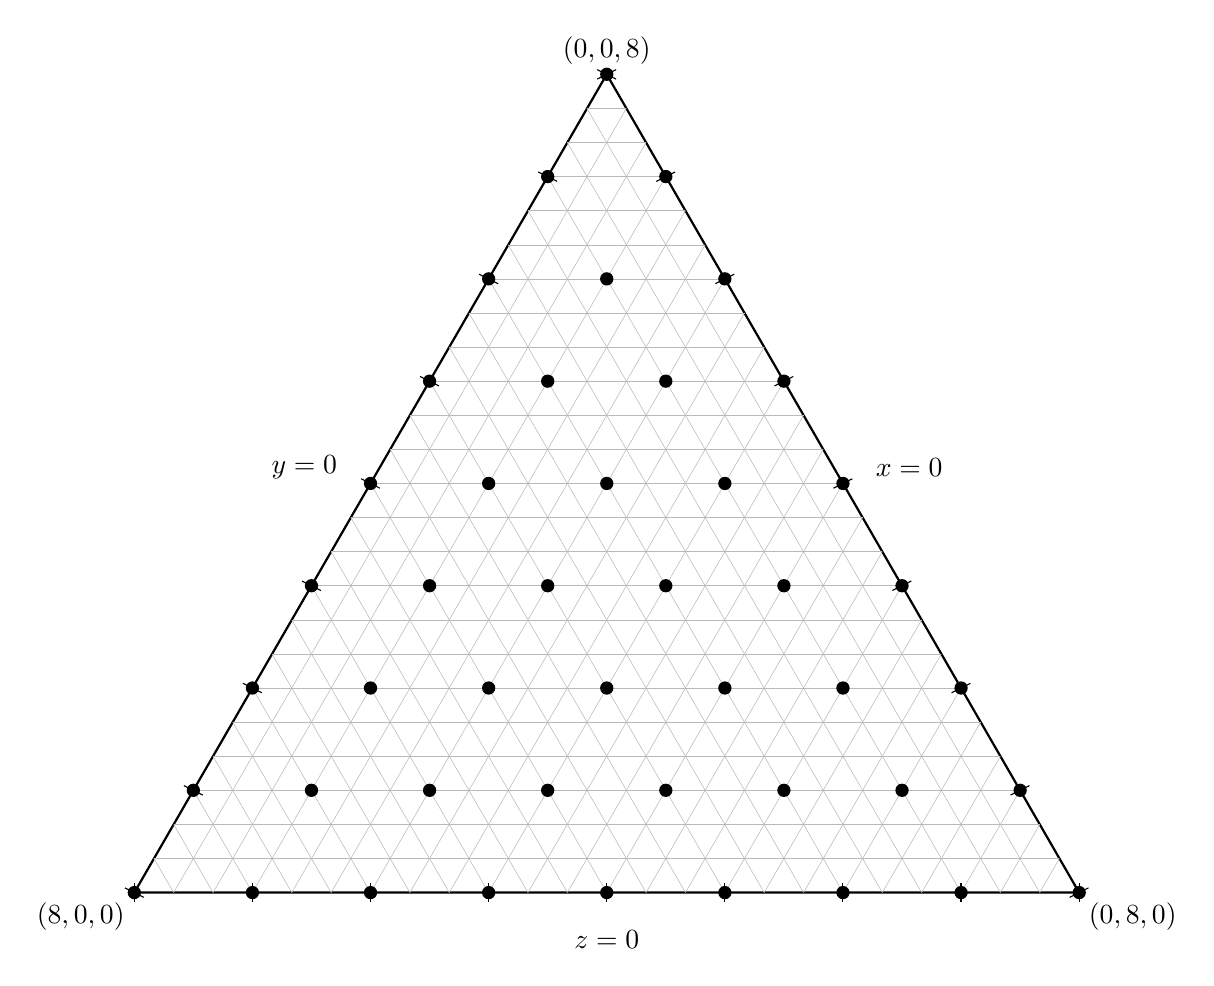
\begin{tikzpicture}[scale=12]

% ----- Parameters -----
\def\N{8} % sum of coordinates

% ----- Triangle vertices -----
\coordinate (X) at (0,0);                 % (8,0,0)
\coordinate (Y) at (1,0);                 % (0,8,0)
\coordinate (Z) at (0.5,{sqrt(3)/2});    % (0,0,8)

% ----- Outline -----
\draw[thick] (X)--(Y)--(Z)--cycle;


% ----- Grid ------


  % grid lines: three families
  \foreach \k in {1,...,23} {
    \pgfmathsetmacro{\t}{\k/24}

    % parallel to YZ
    \draw[very thin, gray!55] ($(X)!\t!(Y)$) -- ($(X)!\t!(Z)$);

    % parallel to XZ
    \draw[very thin, gray!55] ($(X)!\t!(Y)$) -- ($(Z)!\t!(Y)$);

    % parallel to XY
    \draw[very thin, gray!55] ($(X)!\t!(Z)$) -- ($(Y)!\t!(Z)$);
  }

% ----- Integer lattice points -----
\foreach \x in {0,...,\N} {
  \foreach \y in {0,...,\N} {
    \pgfmathtruncatemacro{\z}{\N-\x-\y}
    \ifnum\z<0\relax
    \else
      % barycentric -> Cartesian
      \pgfmathsetmacro{\px}{(\y + 0.5*\z)/\N}
      \pgfmathsetmacro{\py}{(sqrt(3)/2)*(\z/\N)}
      \fill (\px,\py) circle[radius=0.2pt];
    \fi
  }
}

% ----- Tick marks + labels -----

% Edge XY  (z = 0)
\foreach \i in {0,...,\N} {
  \pgfmathsetmacro{\t}{\i/\N}
  \coordinate (P) at ($(X)!\t!(Y)$);
  \draw ($(P)+(0,0.01)$)--($(P)-(0,0.01)$);
  %\node[below] at (P) {\small $\i$};
}

% Edge XZ  (y = 0)
\foreach \i in {0,...,\N} {
  \pgfmathsetmacro{\t}{\i/\N}
  \coordinate (P) at ($(X)!\t!(Z)$);
  \draw ($(P)+(-0.01,0.005)$)--($(P)+(0.01,-0.005)$);
  %\node[left] at (P) {\small $\i$};
}

% Edge YZ  (x = 0)
\foreach \i in {0,...,\N} {
  \pgfmathsetmacro{\t}{\i/\N}
  \coordinate (P) at ($(Y)!\t!(Z)$);
  \draw ($(P)+(0.01,0.005)$)--($(P)+(-0.01,-0.005)$);
  %\node[right] at (P) {\small $\i$};
}

% ----- Axis / vertex labels -----
\node[below left]  at (X) {$(8,0,0)$};
\node[below right] at (Y) {$(0,8,0)$};
\node[above]       at (Z) {$(0,0,8)$};

\node at (0.5,-0.05) {$z=0$};
\node at (0.18,0.45) {$y=0$};
\node at (0.82,0.45) {$x=0$};

%\node at (0.5,0.35) {$x+y+z=8$};

\end{tikzpicture}

\vfill




\end{document}